\documentclass{article}
\usepackage[a4paper, total={6in, 27cm}]{geometry}
\usepackage{amsmath}
\usepackage{graphicx}
\usepackage{tcolorbox}
\usepackage[makeroom]{cancel}

\begin{document}

\title{MATH 340}
\author{Quiz 1 Solutions}
\date{\today}
\maketitle

\begin{enumerate}
	\item (5 points) True of False
		\begin{enumerate}
			\item $\xcancel{\text{(T)}}$  (F)  The constant function $y'(x)=\pi$ is a
				solution of the ODE $y'(x)=x\sin^2(y)$.
			\item $\xcancel{\text{(T)}}$  (F)  For the initial value problem
				$\begin{cases}
					x'(t)=2x+e^t\\
					x(0)=0
				\end{cases}$, the solution is $x(t)=e^{2t}-e^t$.
			\item (T)  $\xcancel{\text{(F)}}$  The ODE $x'(t)+\sin(x(t))=0$ is linear.
			\item (T)  $\xcancel{\text{(F)}}$  The ODE $x'(t)+\sin^2(x(t))=0$ is of order 2.
			\item $\xcancel{\text{(T)}}$  (F)  The ODE $x'(t)+2tx(t)=0$ is linear.
		\end{enumerate}
	\item (5 points) The direction field of an ODE is shown below.

		\begin{center}
		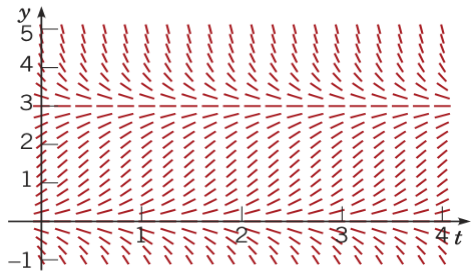
\includegraphics[width=0.5\textwidth]{quiz1DirField.png}
		\end{center}
		\begin{enumerate}
			\item Circle the differential equation that corresponds
				to the direction field. Briefly explain why.
			\[
				y'=y(y-3);\quad \boxed{y'=y(3-y)};\quad y'=y-3;\quad y'=y.
			\]
			\begin{minipage}[t][5cm][t]{0.8\textwidth}
				We clearly have 2 zeros which are $y=0$ and
				$y=3$ so it has to be one of the first 2
				options. Then we see that in order to match the
				sign of $y'$ we need to pick the second.
			\end{minipage}
			\item Based on the diagram identify two equilibrium
				points of the ODE (i.e. where the function
				stays constant).

			The equilibrim solutions are $y=0$ and $y=3$.
		\end{enumerate}
	\newpage
\item (10 points) Consider the initial value problem
	$\begin{cases}
		Q'(t)+\frac{r}{100}Q(t)=\frac{r}{4}\\
		Q(0)=Q_0
	\end{cases}$
	with two positive parameters $r,Q_0$ (this means they are constant!).
	\begin{enumerate}
		\item Find the solution to the IVP.
		\item Find the limit of the solution as $t\to\infty$. (That is
			if $Q_{IVP}(t)$ is the solution you found, then compute
			$\lim_{t\to\infty}Q_{IVP}(t)$).
	\end{enumerate}

	(a)
	This is of the form $\frac{dy}{dt}=ay-b$ so we can use the general formula to get:
	\[
		Q_{IVP}(t)=\frac{-\frac{r}{4}}{-\frac{r}{100}}+
		\left(Q_0-\frac{-\frac{r}{4}}{-\frac{r}{100}}\right)e^{-\frac{r}{100}t}
		=25+(Q_0-25)e^{-rt/100}.
	\]

	(b)
	Notice that $(Q_0-25)e^{-rt/100}\to0$ as $t\to\infty$, because the
	exponential goes to 0.
	\[
		\lim_{t\to\infty}Q_{IVP}(t)=25.
	\]
\end{enumerate}

\end{document}
